\documentclass[a4paper,12pt,one side,titlepage]{report}


%en francais
\usepackage[T1]{fontenc}
\usepackage{lmodern}
\usepackage[utf8]{inputenc}
\usepackage[francais]{babel}



\usepackage{listings}
\usepackage{geometry}
\usepackage{graphicx}
\usepackage{eurosym}
\usepackage{url}
\usepackage{pdfpages}
\usepackage[acronym]{glossaries}
\usepackage{hyperref}
\usepackage{graphicx}
%\usepackage[top=2.5cm,bottom=2.5cm,left=2.5cm,right=2.5cm]{geometry}
%\hypersetup{pdfborder=0}




\newglossaryentry{firewall}
{
	name={firewall},
	description={Protection pour serveur}
}

\newglossaryentry{naxsi}
{
	name={naxsi},
	description={Un type de firewall}
}



\makeglossaries
\begin{document}
%\includepdf[pages = {1-1}]{./pdf/1stpage.pdf}
%\includepdf[pages = {1-1}]{./pdf/pagegarde.pdf}


\begin{titlepage}
\begin{center}

\textsc{\LARGE Licence ASRALL}\\[1.5cm]

\textsc{\Large Exposé technique}\\[5.9cm]

% Title
{ \huge \bfseries Fully Automatic Installation\\[1.9cm] }

% Author and supervisor
\noindent
\begin{minipage}{0.4\textwidth}
\begin{flushleft} \large
François \textsc{Dupont}
\end{flushleft}
\end{minipage}%
\begin{minipage}{0.4\textwidth}
\begin{flushright} \large
Florent \textsc{Fillion}
\end{flushright}
\end{minipage}

\vfill

% Bottom of the page
{\large \today}

\end{center}
\end{titlepage}


%Page table des matières
\tableofcontents

%Introduction
\chapter{Introduction}
\section{Objectifs}
\subsection{Définition}
\textit{Fully Automatic Installation} ou \textsc{FAI} est un logiciel libre, inspiré de son équivalent \textsc{Solaris}, \textsc{Jumpstart}. Il permet d'installer et de configurer un système d'exploitation Linux sur une ou plusieurs machines, en utilisant un infrastructure client serveur, de façon rapide et automatisé.

Il est à noter que \textsc{FAI} n'est pas interactif contrairement à d'autres logiciels remplissant sensiblement la même fonction. Ce logiciel est également considéré comme mature (il en est à sa 4\textsuperscript{ème} itération majeure (4.0) et est développé de façon continue depuis 1999.

\subsection{Utilité}
\textsc{FAI} s'adresse particulièrement aux administrateurs ayant à gérer un grand parc de machine sous Linux, que ce parc soit \textit{virtualisé} ou physique (et même des \textit{chroot}s).

\section{Histoire}


\section{Concepts}
Cette partie pourrait avoir sa place dans le chapitre traitant de la technique à proprement parler, cependant, il nous semble essentiel d'exposer les principes fondamentaux (et simples une fois assimilés) de \textsc{FAI}.



\chapter{Technique}

\chapter{Alternatives}
Il existe plusieurs alternatives à FAI, tels que Jumpstart(Solaris), Kickstart(RedHat), Rembo, ou encore ...................

\section{Jumpstart}
......................

\section{Kickstart}
Kickstart a été créé par RedHat afin d'automatiser l'installation de Fedora et Red Hate Enterprise Linux. Sa configuration s'effectue dans un fichier texte unique contenant une liste d'éléments, chacun identifié par un mot-clé. Ces éléments correspondent aux réponses à toutes les questions qui devraient normalement être posées lors d'une installation typique.\\
Ce fichier peut être créé manuellement en partant d'un fichier vierge puis en écrivant les directives une par une.
Cependant, et contrairement à FAI, il existe une interface utilisateur graphique, "Kickstart Configuration", permettant ainsi une configuration plus simple puisque il n'est pas nécessaire de se rappeler de la syntaxe exacte des fichiers :\\
\begin{center}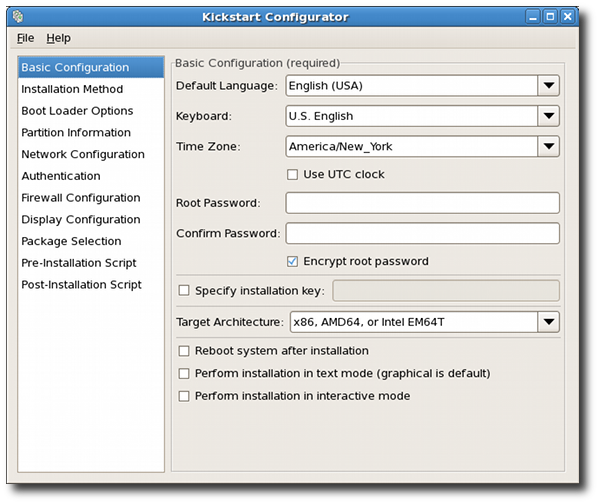
\includegraphics[scale=0.5]{./img/kickstart.png}\end{center}
.......................

\section{Rembo}
Rembo est le successeur de BPBatch. C’est un environnement commercial de création et de déploiement d’images sur PC. Le serveur Rembo peut s’exécuter sur Windows, Linux, ou encore FreeBSD et s’appuie sur un serveur DHCP. Les machines clientes doivent donc supporter PXE. Les clients du réseau sont répartis en plusieurs groupes, ce qui permet de définir des comportements par type de machine, par salle, ... 

\chapter{Sources}
http://fai-project.org/

\end{document}
